% Options for packages loaded elsewhere
\PassOptionsToPackage{unicode}{hyperref}
\PassOptionsToPackage{hyphens}{url}
\PassOptionsToPackage{dvipsnames,svgnames,x11names}{xcolor}
%
\documentclass[
  a4paper,
  DIV=11,
  numbers=noendperiod]{scrartcl}

\usepackage{amsmath,amssymb}
\usepackage{iftex}
\ifPDFTeX
  \usepackage[T1]{fontenc}
  \usepackage[utf8]{inputenc}
  \usepackage{textcomp} % provide euro and other symbols
\else % if luatex or xetex
  \usepackage{unicode-math}
  \defaultfontfeatures{Scale=MatchLowercase}
  \defaultfontfeatures[\rmfamily]{Ligatures=TeX,Scale=1}
\fi
\usepackage{lmodern}
\ifPDFTeX\else  
    % xetex/luatex font selection
\fi
% Use upquote if available, for straight quotes in verbatim environments
\IfFileExists{upquote.sty}{\usepackage{upquote}}{}
\IfFileExists{microtype.sty}{% use microtype if available
  \usepackage[]{microtype}
  \UseMicrotypeSet[protrusion]{basicmath} % disable protrusion for tt fonts
}{}
\makeatletter
\@ifundefined{KOMAClassName}{% if non-KOMA class
  \IfFileExists{parskip.sty}{%
    \usepackage{parskip}
  }{% else
    \setlength{\parindent}{0pt}
    \setlength{\parskip}{6pt plus 2pt minus 1pt}}
}{% if KOMA class
  \KOMAoptions{parskip=half}}
\makeatother
\usepackage{xcolor}
\usepackage[top=20mm,bottom=20mm,left=20mm,right=20mm,heightrounded]{geometry}
\setlength{\emergencystretch}{3em} % prevent overfull lines
\setcounter{secnumdepth}{-\maxdimen} % remove section numbering
% Make \paragraph and \subparagraph free-standing
\ifx\paragraph\undefined\else
  \let\oldparagraph\paragraph
  \renewcommand{\paragraph}[1]{\oldparagraph{#1}\mbox{}}
\fi
\ifx\subparagraph\undefined\else
  \let\oldsubparagraph\subparagraph
  \renewcommand{\subparagraph}[1]{\oldsubparagraph{#1}\mbox{}}
\fi

\usepackage{color}
\usepackage{fancyvrb}
\newcommand{\VerbBar}{|}
\newcommand{\VERB}{\Verb[commandchars=\\\{\}]}
\DefineVerbatimEnvironment{Highlighting}{Verbatim}{commandchars=\\\{\}}
% Add ',fontsize=\small' for more characters per line
\usepackage{framed}
\definecolor{shadecolor}{RGB}{241,243,245}
\newenvironment{Shaded}{\begin{snugshade}}{\end{snugshade}}
\newcommand{\AlertTok}[1]{\textcolor[rgb]{0.68,0.00,0.00}{#1}}
\newcommand{\AnnotationTok}[1]{\textcolor[rgb]{0.37,0.37,0.37}{#1}}
\newcommand{\AttributeTok}[1]{\textcolor[rgb]{0.40,0.45,0.13}{#1}}
\newcommand{\BaseNTok}[1]{\textcolor[rgb]{0.68,0.00,0.00}{#1}}
\newcommand{\BuiltInTok}[1]{\textcolor[rgb]{0.00,0.23,0.31}{#1}}
\newcommand{\CharTok}[1]{\textcolor[rgb]{0.13,0.47,0.30}{#1}}
\newcommand{\CommentTok}[1]{\textcolor[rgb]{0.37,0.37,0.37}{#1}}
\newcommand{\CommentVarTok}[1]{\textcolor[rgb]{0.37,0.37,0.37}{\textit{#1}}}
\newcommand{\ConstantTok}[1]{\textcolor[rgb]{0.56,0.35,0.01}{#1}}
\newcommand{\ControlFlowTok}[1]{\textcolor[rgb]{0.00,0.23,0.31}{#1}}
\newcommand{\DataTypeTok}[1]{\textcolor[rgb]{0.68,0.00,0.00}{#1}}
\newcommand{\DecValTok}[1]{\textcolor[rgb]{0.68,0.00,0.00}{#1}}
\newcommand{\DocumentationTok}[1]{\textcolor[rgb]{0.37,0.37,0.37}{\textit{#1}}}
\newcommand{\ErrorTok}[1]{\textcolor[rgb]{0.68,0.00,0.00}{#1}}
\newcommand{\ExtensionTok}[1]{\textcolor[rgb]{0.00,0.23,0.31}{#1}}
\newcommand{\FloatTok}[1]{\textcolor[rgb]{0.68,0.00,0.00}{#1}}
\newcommand{\FunctionTok}[1]{\textcolor[rgb]{0.28,0.35,0.67}{#1}}
\newcommand{\ImportTok}[1]{\textcolor[rgb]{0.00,0.46,0.62}{#1}}
\newcommand{\InformationTok}[1]{\textcolor[rgb]{0.37,0.37,0.37}{#1}}
\newcommand{\KeywordTok}[1]{\textcolor[rgb]{0.00,0.23,0.31}{#1}}
\newcommand{\NormalTok}[1]{\textcolor[rgb]{0.00,0.23,0.31}{#1}}
\newcommand{\OperatorTok}[1]{\textcolor[rgb]{0.37,0.37,0.37}{#1}}
\newcommand{\OtherTok}[1]{\textcolor[rgb]{0.00,0.23,0.31}{#1}}
\newcommand{\PreprocessorTok}[1]{\textcolor[rgb]{0.68,0.00,0.00}{#1}}
\newcommand{\RegionMarkerTok}[1]{\textcolor[rgb]{0.00,0.23,0.31}{#1}}
\newcommand{\SpecialCharTok}[1]{\textcolor[rgb]{0.37,0.37,0.37}{#1}}
\newcommand{\SpecialStringTok}[1]{\textcolor[rgb]{0.13,0.47,0.30}{#1}}
\newcommand{\StringTok}[1]{\textcolor[rgb]{0.13,0.47,0.30}{#1}}
\newcommand{\VariableTok}[1]{\textcolor[rgb]{0.07,0.07,0.07}{#1}}
\newcommand{\VerbatimStringTok}[1]{\textcolor[rgb]{0.13,0.47,0.30}{#1}}
\newcommand{\WarningTok}[1]{\textcolor[rgb]{0.37,0.37,0.37}{\textit{#1}}}

\providecommand{\tightlist}{%
  \setlength{\itemsep}{0pt}\setlength{\parskip}{0pt}}\usepackage{longtable,booktabs,array}
\usepackage{calc} % for calculating minipage widths
% Correct order of tables after \paragraph or \subparagraph
\usepackage{etoolbox}
\makeatletter
\patchcmd\longtable{\par}{\if@noskipsec\mbox{}\fi\par}{}{}
\makeatother
% Allow footnotes in longtable head/foot
\IfFileExists{footnotehyper.sty}{\usepackage{footnotehyper}}{\usepackage{footnote}}
\makesavenoteenv{longtable}
\usepackage{graphicx}
\makeatletter
\def\maxwidth{\ifdim\Gin@nat@width>\linewidth\linewidth\else\Gin@nat@width\fi}
\def\maxheight{\ifdim\Gin@nat@height>\textheight\textheight\else\Gin@nat@height\fi}
\makeatother
% Scale images if necessary, so that they will not overflow the page
% margins by default, and it is still possible to overwrite the defaults
% using explicit options in \includegraphics[width, height, ...]{}
\setkeys{Gin}{width=\maxwidth,height=\maxheight,keepaspectratio}
% Set default figure placement to htbp
\makeatletter
\def\fps@figure{htbp}
\makeatother

\usepackage{fancyhdr} \pagestyle{fancy} \usepackage{lastpage}
\KOMAoption{captions}{tablesignature}
\makeatletter
\@ifpackageloaded{tcolorbox}{}{\usepackage[skins,breakable]{tcolorbox}}
\@ifpackageloaded{fontawesome5}{}{\usepackage{fontawesome5}}
\definecolor{quarto-callout-color}{HTML}{909090}
\definecolor{quarto-callout-note-color}{HTML}{0758E5}
\definecolor{quarto-callout-important-color}{HTML}{CC1914}
\definecolor{quarto-callout-warning-color}{HTML}{EB9113}
\definecolor{quarto-callout-tip-color}{HTML}{00A047}
\definecolor{quarto-callout-caution-color}{HTML}{FC5300}
\definecolor{quarto-callout-color-frame}{HTML}{acacac}
\definecolor{quarto-callout-note-color-frame}{HTML}{4582ec}
\definecolor{quarto-callout-important-color-frame}{HTML}{d9534f}
\definecolor{quarto-callout-warning-color-frame}{HTML}{f0ad4e}
\definecolor{quarto-callout-tip-color-frame}{HTML}{02b875}
\definecolor{quarto-callout-caution-color-frame}{HTML}{fd7e14}
\makeatother
\makeatletter
\makeatother
\makeatletter
\makeatother
\makeatletter
\@ifpackageloaded{caption}{}{\usepackage{caption}}
\AtBeginDocument{%
\ifdefined\contentsname
  \renewcommand*\contentsname{Table des matières}
\else
  \newcommand\contentsname{Table des matières}
\fi
\ifdefined\listfigurename
  \renewcommand*\listfigurename{Liste des Figures}
\else
  \newcommand\listfigurename{Liste des Figures}
\fi
\ifdefined\listtablename
  \renewcommand*\listtablename{Liste des Tables}
\else
  \newcommand\listtablename{Liste des Tables}
\fi
\ifdefined\figurename
  \renewcommand*\figurename{Figure}
\else
  \newcommand\figurename{Figure}
\fi
\ifdefined\tablename
  \renewcommand*\tablename{Tableau}
\else
  \newcommand\tablename{Tableau}
\fi
}
\@ifpackageloaded{float}{}{\usepackage{float}}
\floatstyle{ruled}
\@ifundefined{c@chapter}{\newfloat{codelisting}{h}{lop}}{\newfloat{codelisting}{h}{lop}[chapter]}
\floatname{codelisting}{Listing}
\newcommand*\listoflistings{\listof{codelisting}{Liste des Listings}}
\makeatother
\makeatletter
\@ifpackageloaded{caption}{}{\usepackage{caption}}
\@ifpackageloaded{subcaption}{}{\usepackage{subcaption}}
\makeatother
\makeatletter
\@ifpackageloaded{tcolorbox}{}{\usepackage[skins,breakable]{tcolorbox}}
\makeatother
\makeatletter
\@ifundefined{shadecolor}{\definecolor{shadecolor}{rgb}{.97, .97, .97}}
\makeatother
\makeatletter
\makeatother
\makeatletter
\makeatother
\ifLuaTeX
\usepackage[bidi=basic]{babel}
\else
\usepackage[bidi=default]{babel}
\fi
\babelprovide[main,import]{french}
% get rid of language-specific shorthands (see #6817):
\let\LanguageShortHands\languageshorthands
\def\languageshorthands#1{}
\ifLuaTeX
  \usepackage{selnolig}  % disable illegal ligatures
\fi
\IfFileExists{bookmark.sty}{\usepackage{bookmark}}{\usepackage{hyperref}}
\IfFileExists{xurl.sty}{\usepackage{xurl}}{} % add URL line breaks if available
\urlstyle{same} % disable monospaced font for URLs
\hypersetup{
  pdftitle={Recherche dichotomique dans un tableau trié},
  pdflang={fr},
  colorlinks=true,
  linkcolor={blue},
  filecolor={Maroon},
  citecolor={Blue},
  urlcolor={Blue},
  pdfcreator={LaTeX via pandoc}}

\title{Recherche dichotomique dans un tableau trié}
\usepackage{etoolbox}
\makeatletter
\providecommand{\subtitle}[1]{% add subtitle to \maketitle
  \apptocmd{\@title}{\par {\large #1 \par}}{}{}
}
\makeatother
\subtitle{S6 - Algorithmique (1)}
\author{}
\date{}

\begin{document}
\maketitle
\lhead{Spécialité NSI} \rhead{Première} \chead{} \cfoot{} \lfoot{Lycée \'Emile Duclaux} \rfoot{Page \thepage/\pageref{LastPage}} \renewcommand{\headrulewidth}{0pt} \renewcommand{\footrulewidth}{0pt} \thispagestyle{fancy} \vspace{-2cm}

\ifdefined\Shaded\renewenvironment{Shaded}{\begin{tcolorbox}[borderline west={3pt}{0pt}{shadecolor}, sharp corners, interior hidden, breakable, enhanced, boxrule=0pt, frame hidden]}{\end{tcolorbox}}\fi

On s'intéresse ici au problème de la recherche d'une valeur dans un
tableau que l'on supposera \textbf{triée} dans l'ordre croissant.

\hypertarget{approche-nauxefve}{%
\subsection{1. Approche naïve}\label{approche-nauxefve}}

La première idée qui peut venir à l'esprit est de considérer les
éléments du tableau les uns après les autres et de les comparer avec
l'élément recherché.

On peut ainsi écrire une fonction \texttt{recherche\_naive} qui prend en
paramètre un tableau \texttt{tàbleau} et une valeur \texttt{valeur} et
qui renvoie l'indice de la première occurrence de \texttt{valeur} dans
\texttt{tableau} ou \texttt{-1} si \texttt{valeur} n'est pas dans
\texttt{tableau}.

\begin{Shaded}
\begin{Highlighting}[]
\KeywordTok{def}\NormalTok{ recherche\_naive(tableau, valeur):}
    \ControlFlowTok{for}\NormalTok{ i }\KeywordTok{in} \BuiltInTok{range}\NormalTok{(}\BuiltInTok{len}\NormalTok{(tableau)):}
        \ControlFlowTok{if}\NormalTok{ tableau[i] }\OperatorTok{==}\NormalTok{ valeur:}
            \ControlFlowTok{return}\NormalTok{ i}
    \ControlFlowTok{return} \OperatorTok{{-}}\DecValTok{1}
\end{Highlighting}
\end{Shaded}

Test de cette fonction :

\begin{Shaded}
\begin{Highlighting}[]
\NormalTok{recherche\_naive([}\DecValTok{1}\NormalTok{, }\DecValTok{2}\NormalTok{, }\DecValTok{3}\NormalTok{, }\DecValTok{4}\NormalTok{, }\DecValTok{5}\NormalTok{], }\DecValTok{3}\NormalTok{)}
\end{Highlighting}
\end{Shaded}

\begin{verbatim}
2
\end{verbatim}

\begin{Shaded}
\begin{Highlighting}[]
\NormalTok{recherche\_naive([}\DecValTok{1}\NormalTok{, }\DecValTok{2}\NormalTok{, }\DecValTok{3}\NormalTok{, }\DecValTok{4}\NormalTok{, }\DecValTok{5}\NormalTok{], }\DecValTok{6}\NormalTok{)}
\end{Highlighting}
\end{Shaded}

\begin{verbatim}
-1
\end{verbatim}

La complexité dans le pire des cas correspond ici au cas où la valeur
recherchée n'est pas dans la liste. Il faut alors parcourir toutes les
valeurs du tableau et faire \(n\) comparaisons, où \(n\) est la taille
du tableau. L'algorithme naïf a donc une \textbf{complexité linéaire} en
\(\mathcal{O}(n)\).

Il est possible d'être plus efficace en exploitant le fait que la liste
est triée.

\hypertarget{recherche-dichotomique}{%
\subsection{2. Recherche dichotomique}\label{recherche-dichotomique}}

\hypertarget{le-principe}{%
\subsubsection{Le principe}\label{le-principe}}

De façon intuitive, la recherche dichotomique consiste à \textbf{diviser
par deux} la zone de recherche à chaque étape.

On commence par considérer l'ensemble des éléments du tableau. On
regarde ensuite la valeur de l'élément du \textbf{milieu} du tableau. Si
cette valeur est inférieure à la valeur recherchée, alors on poursuit la
recherche sur la moitié supérieure du tableau. Si la valeur est
supérieure à la valeur recherchée, alors on poursuit la recherche sur la
moitié inférieure. Si la valeur est égale à la valeur recherchée, on a
trouvé l'élément recherché.

\begin{tcolorbox}[enhanced jigsaw, bottomrule=.15mm, colback=white, breakable, title=\textcolor{quarto-callout-important-color}{\faExclamation}\hspace{0.5em}{Principe de l'algorithme}, leftrule=.75mm, opacityback=0, colframe=quarto-callout-important-color-frame, toprule=.15mm, left=2mm, coltitle=black, titlerule=0mm, colbacktitle=quarto-callout-important-color!10!white, rightrule=.15mm, bottomtitle=1mm, opacitybacktitle=0.6, toptitle=1mm, arc=.35mm]

\begin{itemize}
\tightlist
\item
  On considère le tableau \texttt{tableau} trié dans l'ordre croissant
  dans lequel on recherche la valeur \texttt{valeur}.
\item
  On définit les bornes \texttt{gauche} et \texttt{droite} du tableau :
  indices du premier et du dernier élément de la partie du tableau dans
  laquelle on recherche.
\item
  Tant que \texttt{gauche} est inférieur ou égal à \texttt{droite} :

  \begin{itemize}
  \tightlist
  \item
    On calcule l'indice \texttt{milieu} du milieu du tableau.
  \item
    Si \texttt{tableau{[}milieu{]}} est égal à \texttt{valeur}, on
    renvoie \texttt{milieu}.
  \item
    Si \texttt{tableau{[}milieu{]}} est inférieur à \texttt{valeur}, on
    met à jour \texttt{gauche} à \texttt{milieu\ +\ 1}. Lors de
    l'itération suivante, on ne considèrera donc que la partie du
    tableau située à droite de \texttt{milieu}.
  \item
    Si \texttt{tableau{[}milieu{]}} est supérieur à \texttt{valeur}, on
    met à jour \texttt{droite} à \texttt{milieu\ -\ 1}. Lors de
    l'itération suivante, on ne considèrera donc que la partie du
    tableau située à gauche de \texttt{milieu}.
  \end{itemize}
\item
  On renvoie \texttt{-1} si \texttt{valeur} n'est pas dans
  \texttt{tableau}.
\end{itemize}

\end{tcolorbox}

\textbf{Exemple}

On considère le tableau \texttt{{[}1,4,7,10,13,16,19,22,25{]}} et on
cherche la valeur \texttt{22}.

On commence par considérer l'ensemble des éléments du tableau
(\texttt{gauche=0} et \texttt{droite=8}). On regarde ensuite la valeur
de l'élément du \textbf{milieu} du tableau. Ici, il s'agit de l'élément
d'indice 4 (\texttt{milieu=4}), qui vaut 13. La valeur recherchée est
supérieure à 13, donc on ne considère que la partie du tableau située à
droite de l'élément du milieu.

On répète alors l'opération sur la partie du tableau située à droite de
l'élément du milieu (\texttt{gauche=5} et \texttt{droite=8}). On obtient
le tableau \texttt{{[}16,19,22,25{]}} et on cherche la valeur
\texttt{22}. L'élément du milieu de ce tableau vaut 19
(\texttt{milieu=6}), qui est inférieur à 22. On ne considère donc que la
partie du tableau située à droite de l'élément du milieu.

On répète donc l'opération sur la partie du tableau située à droite
(\texttt{gauche=7} et \texttt{droite=8}). On obtient le tableau
\texttt{{[}22,25{]}} et on cherche la valeur \texttt{22}. L'élément du
milieu de ce tableau vaut 22 (\texttt{milieu=7}), qui est égal à 22. On
a donc trouvé la valeur recherchée et l'algorithme est terminé en trois
étapes.

\begin{figure}

{\centering 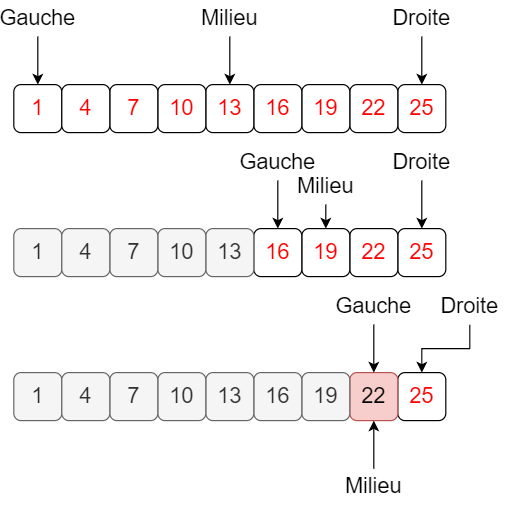
\includegraphics{./recherche_dicho.png}

}

\caption{Recherche dichotomique}

\end{figure}

\hypertarget{programmation}{%
\subsubsection{Programmation}\label{programmation}}

Écrivons une fonction \texttt{recherche\_dichotomique} qui prend en
paramètre un tableau \texttt{tableau} et une valeur \texttt{valeur} et
qui renvoie l'indice d'une occurrence de \texttt{valeur} dans
\texttt{tableau} ou \texttt{-1} si \texttt{valeur} n'est pas dans
\texttt{tableau}.

\begin{Shaded}
\begin{Highlighting}[]
\KeywordTok{def}\NormalTok{ recherche\_dichotomique(tableau, valeur):}
\NormalTok{    gauche }\OperatorTok{=} \DecValTok{0}
\NormalTok{    droite }\OperatorTok{=} \BuiltInTok{len}\NormalTok{(tableau) }\OperatorTok{{-}} \DecValTok{1}
    \ControlFlowTok{while}\NormalTok{ gauche }\OperatorTok{\textless{}=}\NormalTok{ droite:}
\NormalTok{        milieu }\OperatorTok{=}\NormalTok{ (gauche }\OperatorTok{+}\NormalTok{ droite) }\OperatorTok{//} \DecValTok{2}
        \ControlFlowTok{if}\NormalTok{ tableau[milieu] }\OperatorTok{==}\NormalTok{ valeur:}
            \ControlFlowTok{return}\NormalTok{ milieu}
        \ControlFlowTok{elif}\NormalTok{ tableau[milieu] }\OperatorTok{\textless{}}\NormalTok{ valeur:}
\NormalTok{            gauche }\OperatorTok{=}\NormalTok{ milieu }\OperatorTok{+} \DecValTok{1}
        \ControlFlowTok{else}\NormalTok{:}
\NormalTok{            droite }\OperatorTok{=}\NormalTok{ milieu }\OperatorTok{{-}} \DecValTok{1}
    \ControlFlowTok{return} \OperatorTok{{-}}\DecValTok{1}
\end{Highlighting}
\end{Shaded}

Test de cette fonction :

\begin{Shaded}
\begin{Highlighting}[]
\NormalTok{recherche\_dichotomique([}\DecValTok{1}\NormalTok{, }\DecValTok{2}\NormalTok{, }\DecValTok{3}\NormalTok{, }\DecValTok{4}\NormalTok{, }\DecValTok{5}\NormalTok{], }\DecValTok{2}\NormalTok{)}
\end{Highlighting}
\end{Shaded}

\begin{verbatim}
1
\end{verbatim}

\begin{Shaded}
\begin{Highlighting}[]
\NormalTok{recherche\_dichotomique([}\DecValTok{1}\NormalTok{, }\DecValTok{2}\NormalTok{, }\DecValTok{3}\NormalTok{, }\DecValTok{4}\NormalTok{, }\DecValTok{5}\NormalTok{], }\DecValTok{6}\NormalTok{)}
\end{Highlighting}
\end{Shaded}

\begin{verbatim}
-1
\end{verbatim}

\hypertarget{preuve-de-terminaison}{%
\subsubsection{Preuve de terminaison}\label{preuve-de-terminaison}}

Pour prouver que l'algorithme se termine, il faut prouver que la boucle
\texttt{while} se termine, et donc que la condition d'arrêt
\texttt{gauche\ \textgreater{}\ droite} finit par être vérifiée
\textbf{ou bien} que la condition
\texttt{tableau{[}milieu{]}\ ==\ valeur} est vérifiée.

Choisissons comme \textbf{variant de boucle} la différence
\texttt{droite\ -\ gauche} et plaçons-nous dans le cas le plus
défavorable où la condition \texttt{tableau{[}milieu{]}\ ==\ valeur}
n'est jamais vérifiée. À chaque passage dans la boucle, soit
\texttt{gauche} est incrémenté de 1, soit \texttt{droite} est décrémenté
de 1. La différence \texttt{droite\ -\ gauche} est donc toujours
diminuée de 1. Au bout d'un nombre fini d'itérations (au maximum égal à
la taille du tableau moins un), la condition notre variant de boucle
devient donc égal à zéro et la boucle se termine.

La terminaison de l'algorithme est donc prouvée.

\hypertarget{preuve-de-correction}{%
\subsubsection{Preuve de correction}\label{preuve-de-correction}}

Considérons la propriété suivante : à chaque étape de l'algorithme, la
valeur recherchée est située dans la partie du tableau située entre les
indices \texttt{gauche} et \texttt{droite} inclus, ou bien elle n'est
pas dans le tableau.

Montrons que cette propriété est un \textbf{invariant de boucle}.
C'est-à-dire que cette propriété est vraie avant l'exécution de la
première itération de la boucle et qu'elle est vraie après l'exécution
de chaque itération de la boucle.

\textbf{Initialisation} : avant l'exécution de la première itération de
la boucle, si la valeur est dans le tableau, alors elle est située dans
la partie du tableau située entre les indices \texttt{gauche} et
\texttt{droite} inclus. En effet, \texttt{gauche} vaut 0 et
\texttt{droite} vaut la taille du tableau moins un, donc la valeur
recherchée est située dans la partie du tableau située entre les indices
0 et la taille du tableau moins un inclus (c'est le tableau entier !).

\textbf{Conservation} : supposons que la propriété est vraie à l'entrée
dans une itération de la boucle \texttt{while}. Il y a trois
possibilités :

\begin{itemize}
\tightlist
\item
  \texttt{tableau{[}milieu{]}\ ==\ valeur} est vérifiée. Dans ce cas, la
  propriété est vraie à la sortie de l'itération de la boucle et
  l'algorithme retourne l'indice attendu.
\item
  \texttt{tableau{[}milieu{]}\ \textless{}\ valeur} est vérifiée. Dans
  ce cas, \texttt{gauche} est incrémenté de 1. La valeur recherchée est
  donc située dans la partie du tableau située entre les indices
  \texttt{gauche} et \texttt{droite} inclus, ou bien elle est absente du
  tableau.
\item
  \texttt{tableau{[}milieu{]}\ \textgreater{}\ valeur} est vérifiée.
  Dans ce cas, \texttt{droite} est décrémenté de 1. La valeur recherchée
  est donc située dans la partie du tableau située entre les indices
  \texttt{gauche} et \texttt{droite} inclus, ou bien elle est absente du
  tableau.
\end{itemize}

\textbf{Conclusion} : la propriété est donc un invariant de boucle.

Deux cas sont à considérer pour conclure. Si le test
\texttt{tableau{[}milieu{]}\ ==\ valeur} est vérifié au cours des
itérations, alors la valeur est trouvée dans le tableau et on retourne
son indice \texttt{milieu} : c'est bien le comportement attendu. Si le
test \texttt{tableau{[}milieu{]}\ ==\ valeur} n'est jamais vérifié,
alors l'algorithme se termine lorsque
\texttt{gauche\ \textgreater{}\ droite}. D'après notre invariant de
boucle, soit la valeur est alors absente du tableau, soit elle est
située dans la partie du tableau située entre les indices
\texttt{gauche} et \texttt{droite} inclus. Mais cette partie du tableau
est un tableau vide \texttt{{[}{]}}. La valeur est donc absente du
tableau et on retourne l'indice \texttt{-1} : c'est bien le comportement
attendu.

L'algorithme est donc correct.

\hypertarget{complexituxe9}{%
\subsubsection{Complexité}\label{complexituxe9}}

Pour évaluer la complexité de cet algorithme, nous allons évaluer le
nombre d'itérations nécessaires en fonction de la taille \(n\) du
tableau, dans le pire des cas, c'est-à-dire lorsque la valeur recherchée
n'est pas dans le tableau.

À chaque étape, la taille du sous-tableau contenant potentiellement la
valeur recherchée est divisée par deux. Au bout de \(k\) étapes, la
taille du sous-tableau est donc de \(\frac{n}{2^k}\) environ. Si la
valeur recherchée n'est pas dans le tableau, alors on finit par arriver
à un tableau de taille 1 et la boucle se termine au tour suivant. Soit
\(k\) le nombre d'itérations nécessaires pour que la taille du
sous-tableau soit de 1. On a donc \(\frac{n}{2^k}\), et par conséquent
\(n=2^k\). On en déduit que \(k=\log_2 n\).

L'algorithme de recherche dichotomique est donc en
\(\mathcal{O}(\log n)\). On parle de \textbf{complexité logarithmique}.
Cette complexité est meilleure que la complexité linéaire.

\begin{tcolorbox}[enhanced jigsaw, bottomrule=.15mm, colback=white, breakable, title=\textcolor{quarto-callout-note-color}{\faInfo}\hspace{0.5em}{Notion de logarithme de base 2}, leftrule=.75mm, opacityback=0, colframe=quarto-callout-note-color-frame, toprule=.15mm, left=2mm, coltitle=black, titlerule=0mm, colbacktitle=quarto-callout-note-color!10!white, rightrule=.15mm, bottomtitle=1mm, opacitybacktitle=0.6, toptitle=1mm, arc=.35mm]

Si \(x\) est une puissance de 2, alors \(\log_2 x\) est égal à
l'\textbf{exposant} de cette puissance. Par exemple, \(\log_2 8 = 3\)
car \(8 = 2^3\).

\end{tcolorbox}

Pour un tableau de départ de taille \(16=2^4\) dans lequel on cherche
une valeur qui n'y est pas, on effectue 4 itérations :

\begin{itemize}
\tightlist
\item
  au premier tour, on divise le tableau en deux parties de taille
  \(8=2^3\) et on cherche dans la partie de gauche (par exemple) ;
\item
  au deuxième tour, on divise la partie de gauche en deux parties de
  taille \(4=2^2\) et on cherche dans la partie de gauche (par exemple)
  ;
\item
  au troisième tour, on divise la partie de gauche en deux parties de
  taille \(2=2^1\) et on cherche dans la partie de gauche (par exemple)
  ;
\item
  au quatrième tour, on divise la partie de gauche en deux parties de
  taille \(1=2^0\) et on cherche dans la partie de gauche (par exemple).
\end{itemize}

On retrouve bien un nombre d'itérations de l'ordre de \(\log_2 n\).

\hypertarget{comparaison-expuxe9rimentale-des-deux-algorithmes}{%
\subsubsection{Comparaison expérimentale des deux
algorithmes}\label{comparaison-expuxe9rimentale-des-deux-algorithmes}}

\begin{Shaded}
\begin{Highlighting}[]
\ImportTok{import}\NormalTok{ timeit}
\ImportTok{import}\NormalTok{ matplotlib.pyplot }\ImportTok{as}\NormalTok{ plt}

\NormalTok{tailles }\OperatorTok{=}\NormalTok{ [i }\ControlFlowTok{for}\NormalTok{ i }\KeywordTok{in} \BuiltInTok{range}\NormalTok{(}\DecValTok{1}\NormalTok{, }\DecValTok{500}\NormalTok{)]}
\NormalTok{temps\_naive }\OperatorTok{=}\NormalTok{ []}
\NormalTok{temps\_dicho }\OperatorTok{=}\NormalTok{ []}
\CommentTok{\# on applique la recherche dans le pire des cas : valeur absente su tableau}
\NormalTok{valeur }\OperatorTok{=} \DecValTok{1000}
\ControlFlowTok{for}\NormalTok{ n }\KeywordTok{in}\NormalTok{ tailles:}
\NormalTok{    temps\_naive.append(timeit.timeit(}
        \StringTok{"recherche\_naive([k for k in range(n)], valeur)"}\NormalTok{,}
        \BuiltInTok{globals}\OperatorTok{=}\BuiltInTok{globals}\NormalTok{(),}
\NormalTok{        number}\OperatorTok{=}\DecValTok{100}
\NormalTok{    ))}
\NormalTok{    temps\_dicho.append(timeit.timeit(}
        \StringTok{"recherche\_dichotomique([k for k in range(n)], valeur)"}\NormalTok{,}
        \BuiltInTok{globals}\OperatorTok{=}\BuiltInTok{globals}\NormalTok{(),}
\NormalTok{        number}\OperatorTok{=}\DecValTok{100}
\NormalTok{    ))}
\NormalTok{plt.plot(tailles,temps\_naive, }\StringTok{\textquotesingle{}b\textquotesingle{}}\NormalTok{, label}\OperatorTok{=}\StringTok{"Recherche naïve"}\NormalTok{)}
\NormalTok{plt.plot(tailles,temps\_dicho, }\StringTok{\textquotesingle{}r\textquotesingle{}}\NormalTok{, label}\OperatorTok{=}\StringTok{"Recherche dichotomique"}\NormalTok{)}
\NormalTok{plt.xlabel(}\StringTok{"Taille du tableau"}\NormalTok{)}
\NormalTok{plt.ylabel(}\StringTok{"Temps d\textquotesingle{}exécution (en secondes)"}\NormalTok{)}
\NormalTok{plt.legend()}
\NormalTok{plt.show()}
\end{Highlighting}
\end{Shaded}

\begin{figure}[H]

{\centering 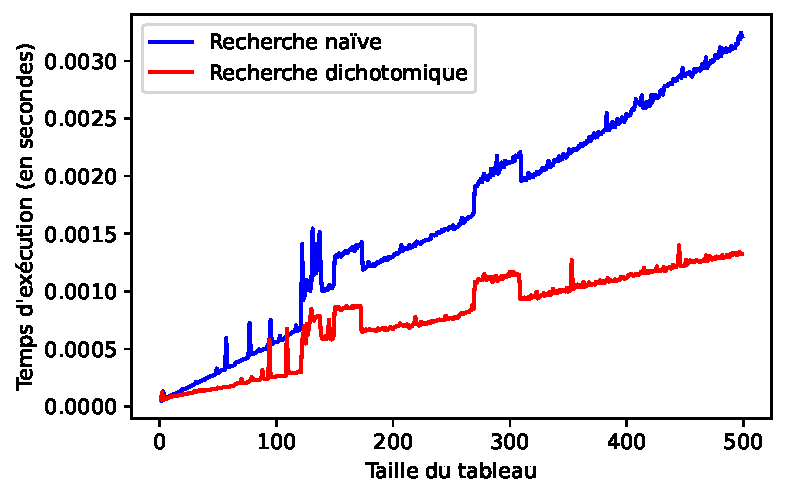
\includegraphics{recherche_files/figure-pdf/cell-8-output-1.pdf}

}

\end{figure}



\end{document}
